\documentclass[journal]{IEEEtran}

\usepackage{cite}
\usepackage{amsmath,amssymb}
\usepackage{graphicx}
\usepackage{booktabs}
\usepackage{url}
\graphicspath{{figures/}}

\begin{document}

\title{AgentRoute: Learning-Based Semantic Capability Routing for AI Agents in Mobile Networks}

\author{\"Omer Faruk Gedikli (220104004103), Bekir Emre Sar{\i}p{\i}nar (220104004039), Bekir G\"oktepe (220104004018)%
\thanks{CSE 476/575 Mobile Communication Networks, Term Project, Fall 2026, Gebze Technical University.}}

\maketitle

\begin{abstract}
% Write the abstract here.
\end{abstract}

\begin{IEEEkeywords}
% Write the keywords here.
\end{IEEEkeywords}

\section{Introduction}
% Write here.

\section{Background and Related Work}
% Write here.

\section{System Design}

\subsection{Capability Addressing}
% Write here.

\subsection{Semantic FIB and Advertisements}
% Write here.

\subsection{Intent-Based Forwarding}
% Write here.

\subsection{Learned Next Hop}
% Write here.

\subsection{Mobility and Handover}
% Write here.

\section{Implementation and Simulation Setup}
% Write here.

\section{Evaluation}

\subsection{Learning Curve}
% Write here.

\begin{figure}[!t]
\centering
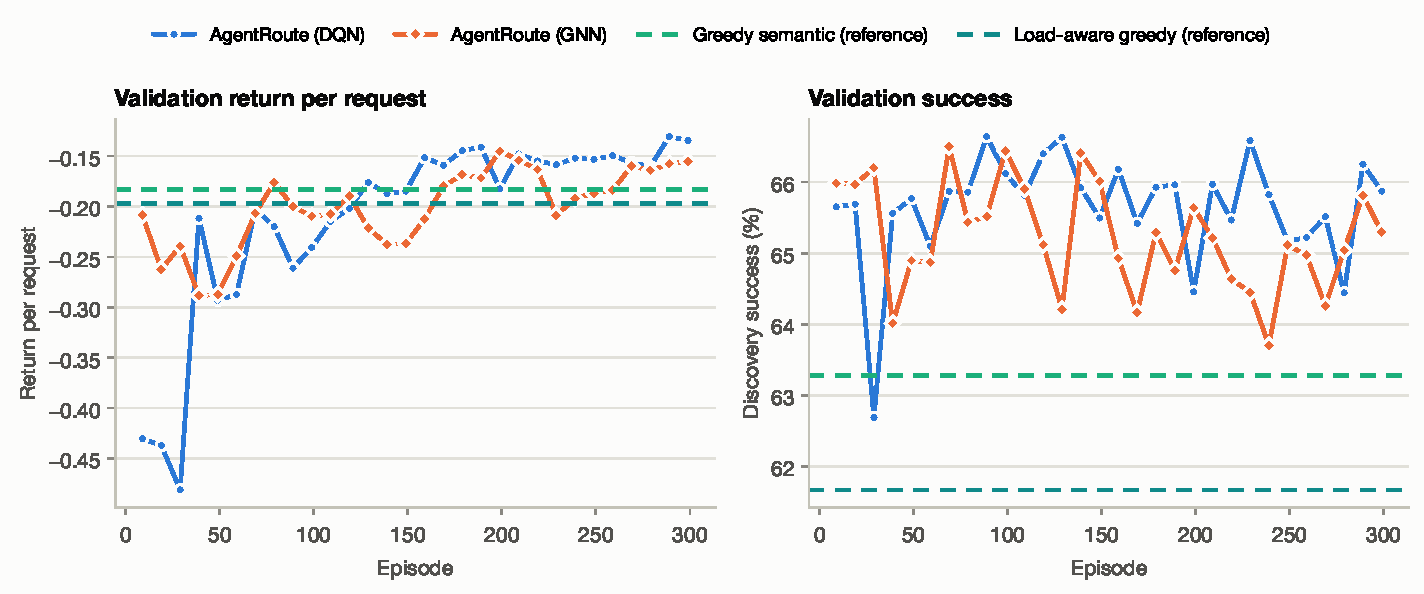
\includegraphics[width=\columnwidth]{learning_curve.pdf}
\caption{Write the caption.}
\label{fig:learning_curve}
\end{figure}

\subsection{Scalability}
% Write here.

\begin{figure}[!t]
\centering
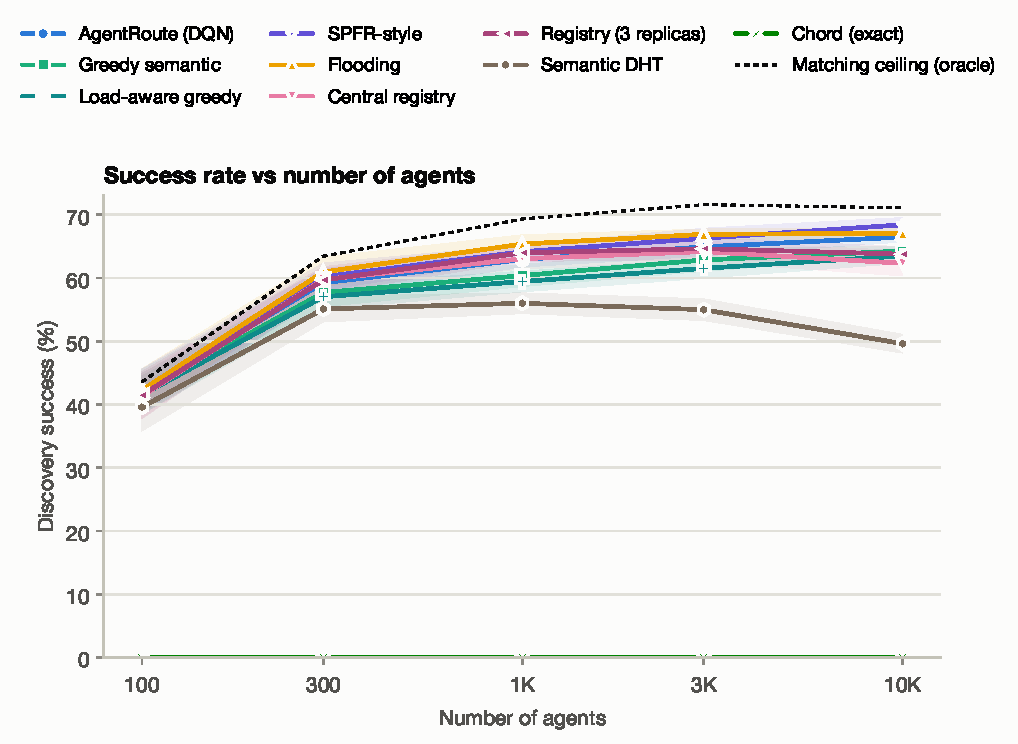
\includegraphics[width=\columnwidth]{scale_success.pdf}
\caption{Write the caption.}
\label{fig:scale_success}
\end{figure}

\begin{figure}[!t]
\centering
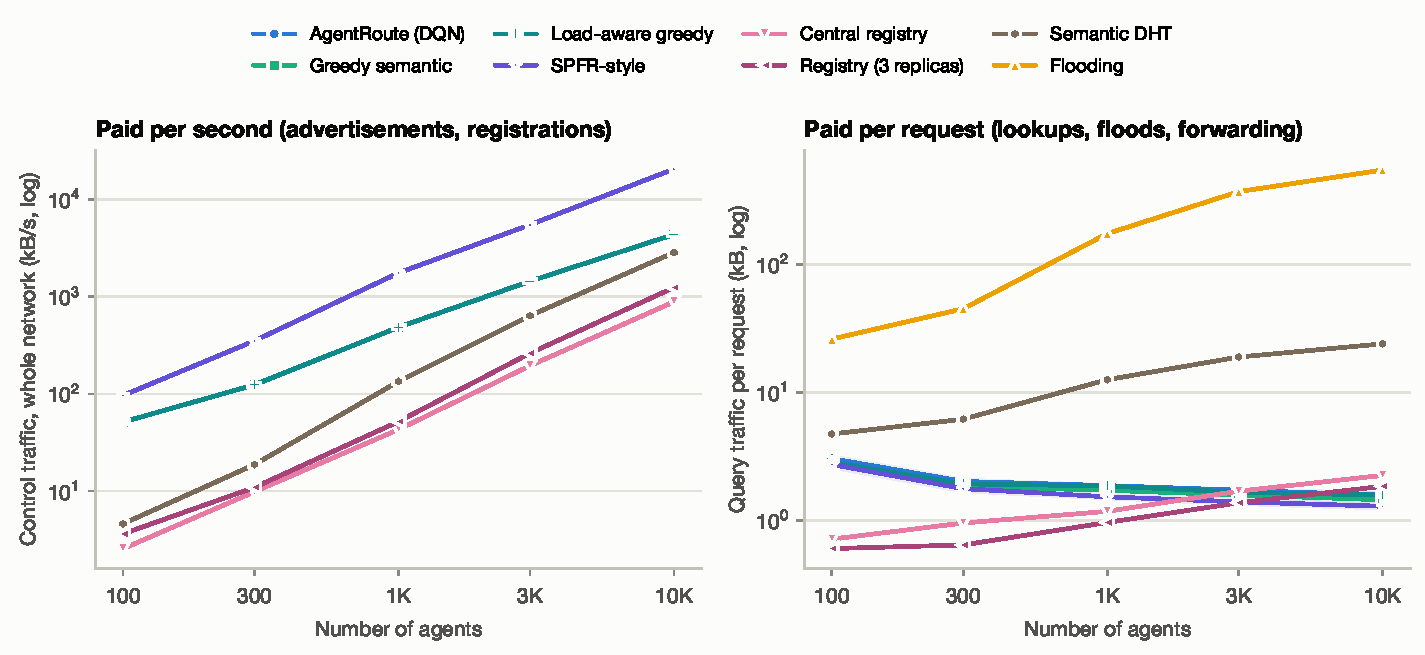
\includegraphics[width=\columnwidth]{scale_overhead.pdf}
\caption{Write the caption.}
\label{fig:scale_overhead}
\end{figure}

\begin{figure}[!t]
\centering
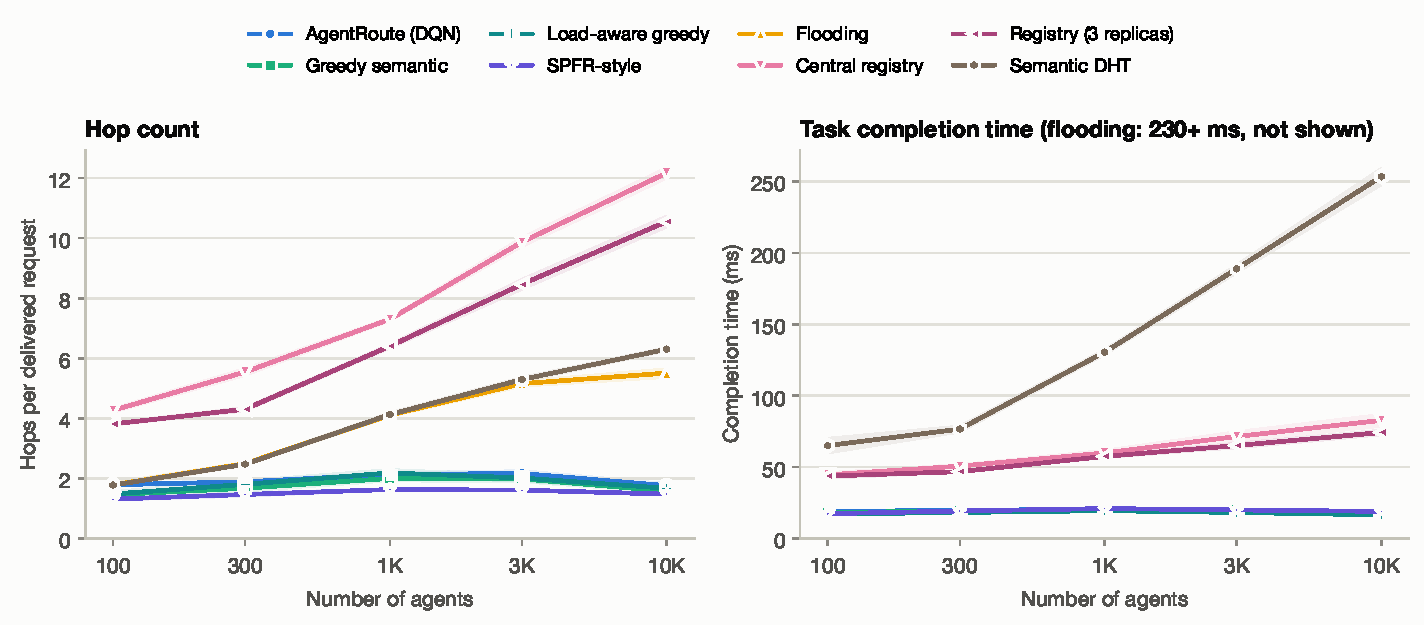
\includegraphics[width=\columnwidth]{scale_hops_time.pdf}
\caption{Write the caption.}
\label{fig:scale_hops_time}
\end{figure}

\subsection{Request Rate and Control Traffic}
% Write here.

\begin{figure}[!t]
\centering
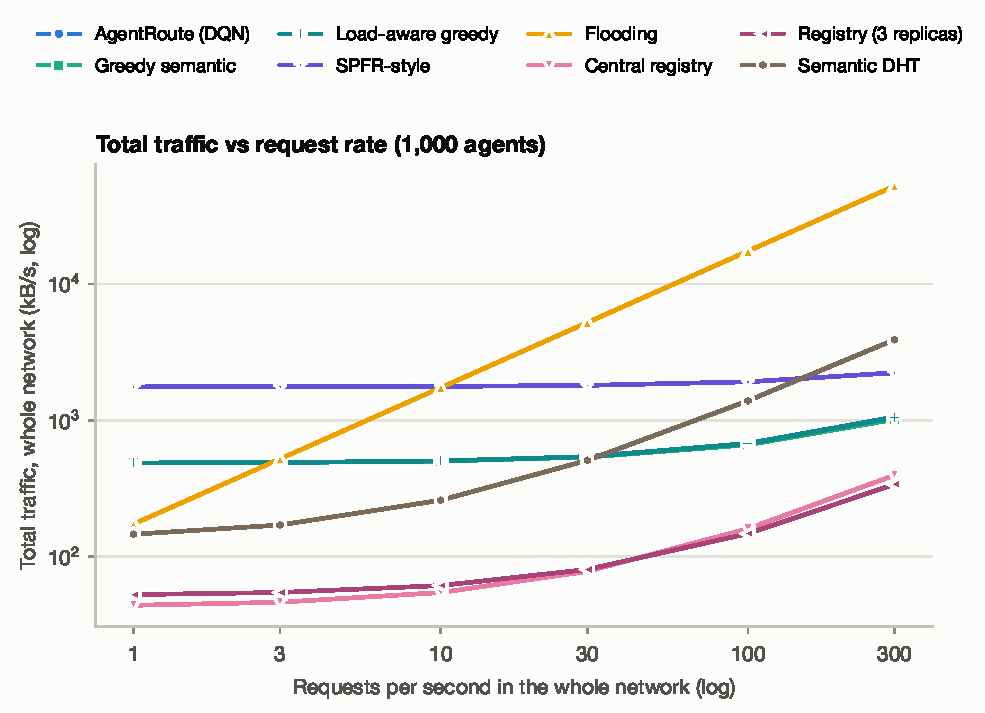
\includegraphics[width=\columnwidth]{rate_crossover.pdf}
\caption{Write the caption.}
\label{fig:rate_crossover}
\end{figure}

\subsection{Mobility}
% Write here.

\begin{figure}[!t]
\centering
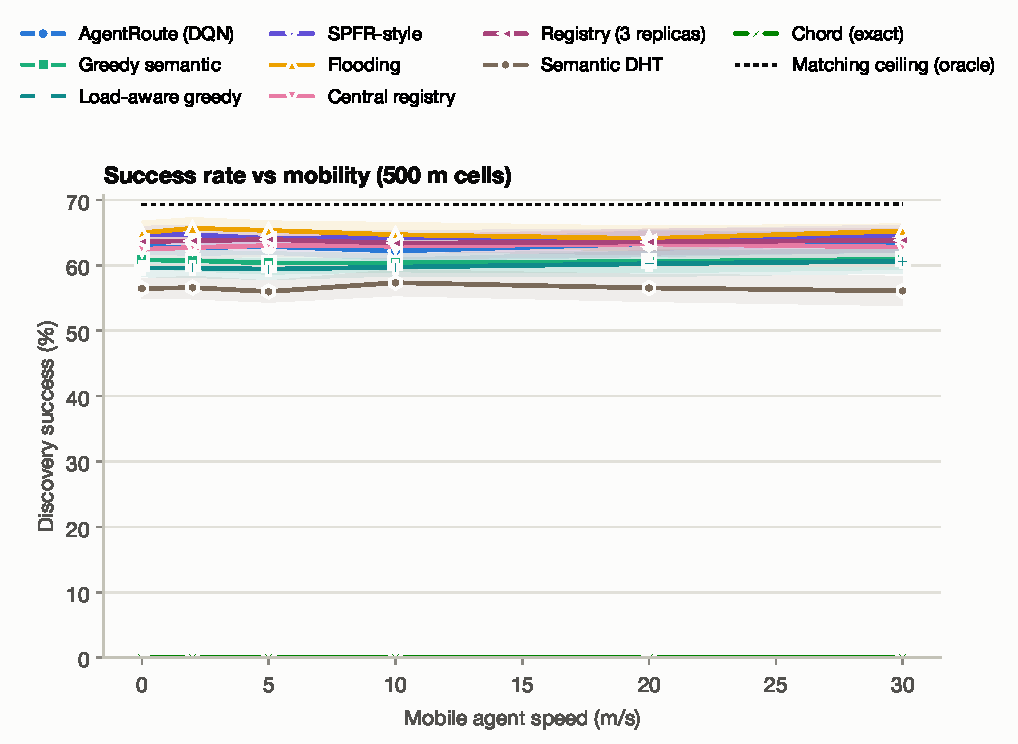
\includegraphics[width=\columnwidth]{mobility_success.pdf}
\caption{Write the caption.}
\label{fig:mobility_success}
\end{figure}

\begin{figure}[!t]
\centering
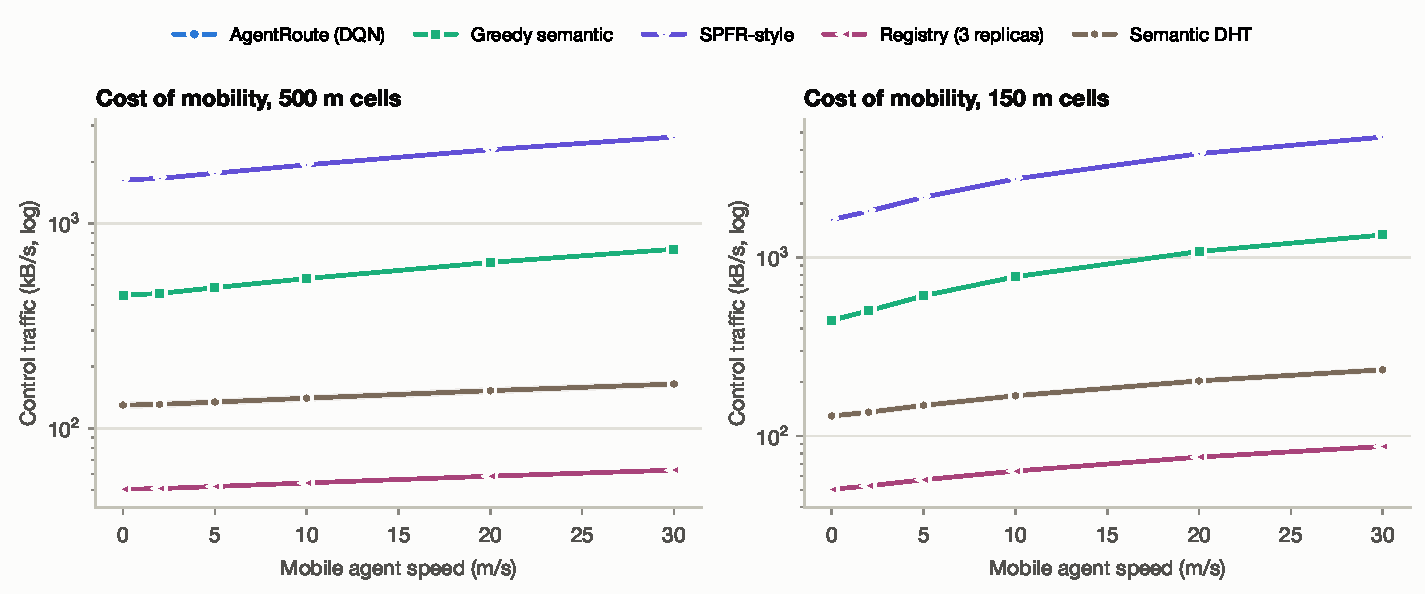
\includegraphics[width=\columnwidth]{mobility_cost.pdf}
\caption{Write the caption.}
\label{fig:mobility_cost}
\end{figure}

\subsection{Node Failure and Load}
% Write here.

\begin{figure}[!t]
\centering
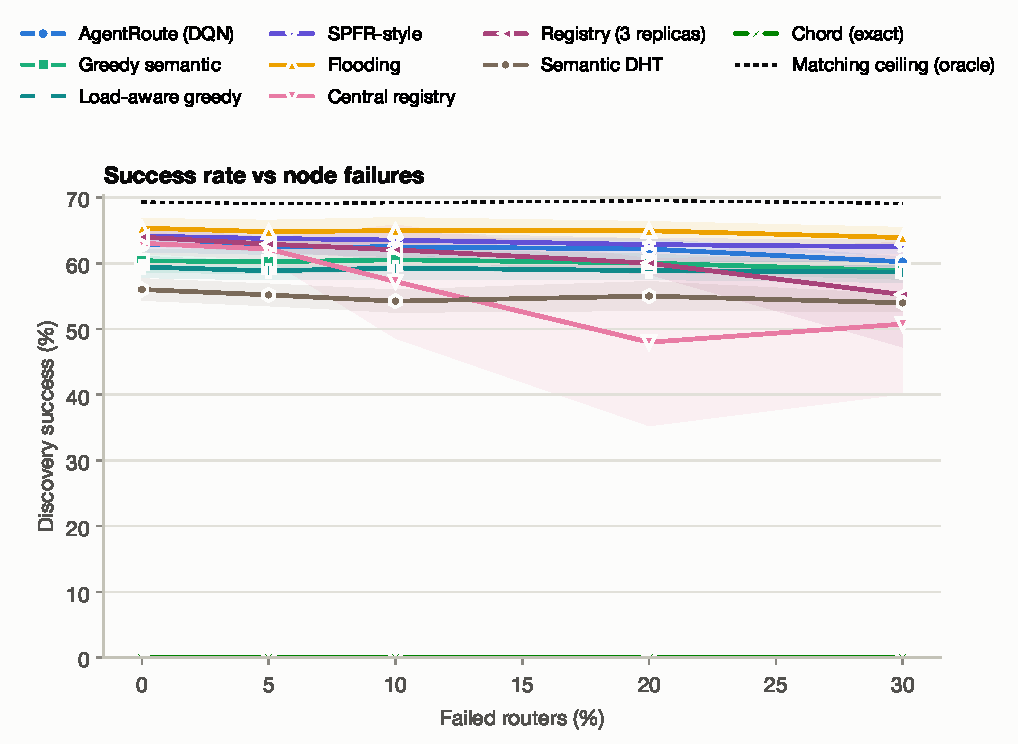
\includegraphics[width=\columnwidth]{failure_success.pdf}
\caption{Write the caption.}
\label{fig:failure_success}
\end{figure}

\begin{figure}[!t]
\centering
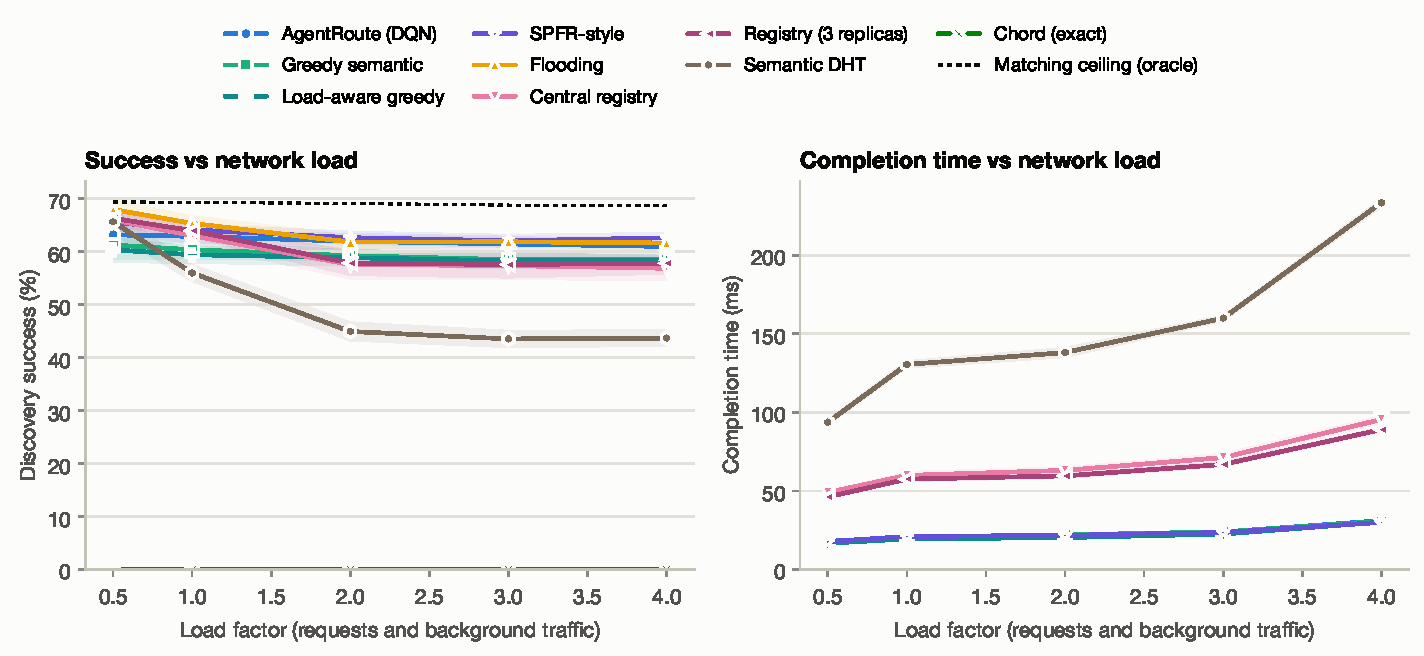
\includegraphics[width=\columnwidth]{load.pdf}
\caption{Write the caption.}
\label{fig:load}
\end{figure}

\subsection{Advertisement Radius}
% Write here.

\begin{figure}[!t]
\centering
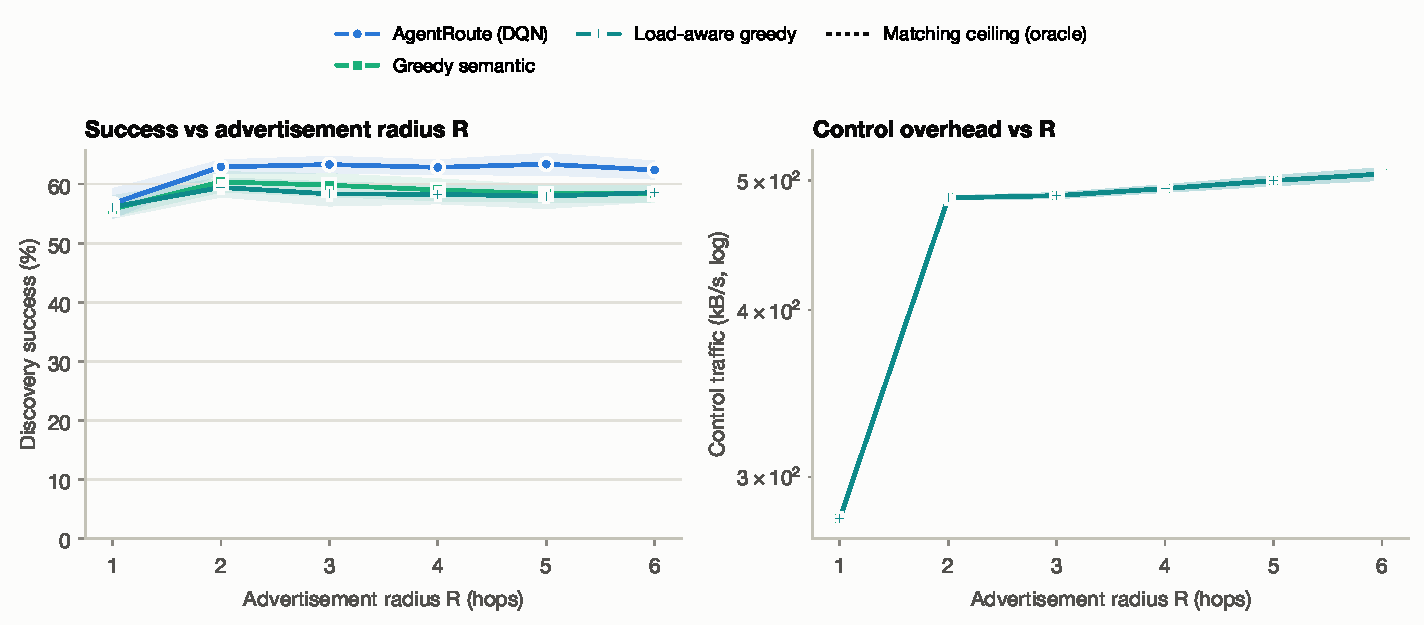
\includegraphics[width=\columnwidth]{radius.pdf}
\caption{Write the caption.}
\label{fig:radius}
\end{figure}

\subsection{Radio Model}
% Write here.

\begin{figure}[!t]
\centering
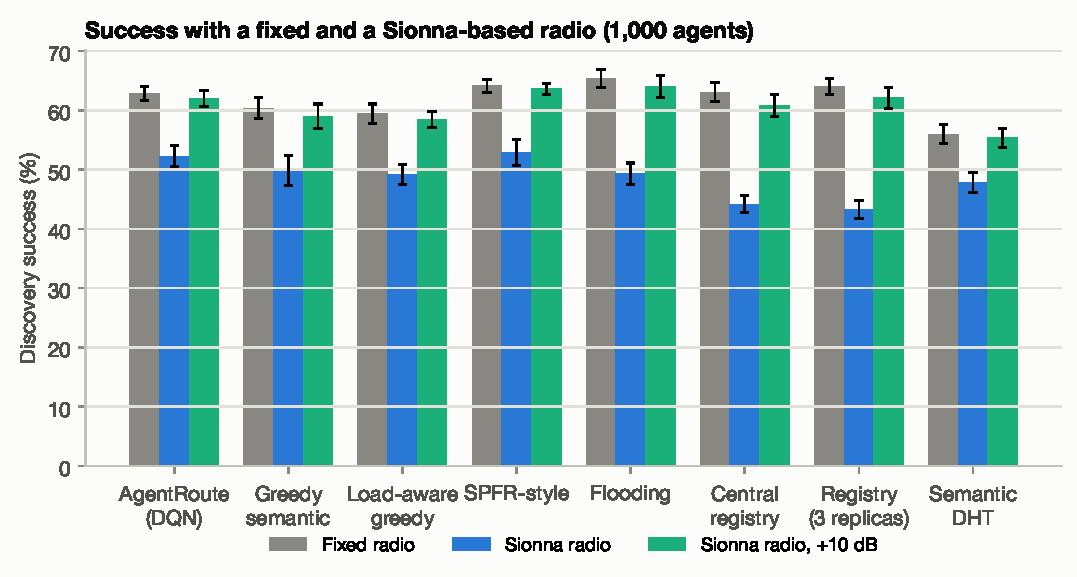
\includegraphics[width=\columnwidth]{radio_compare.pdf}
\caption{Write the caption.}
\label{fig:radio_compare}
\end{figure}

\section{Discussion}
% Write here.

\section{Conclusion}
% Write here.

\section*{Team Contributions}
% Write here.

\begin{thebibliography}{1}

\bibitem{ref1}
Replace this entry with the first reference.

\end{thebibliography}

\end{document}
